%% ----------------------------------------------------------------
%% Thesis.tex -- MAIN FILE (the one that you compile with LaTeX)
%% ---------------------------------------------------------------- 

% Set up the document
\documentclass[a4paper, 11pt, oneside]{Thesis}  % Use the "Thesis" style, based on the ECS Thesis style by Steve Gunn
%\graphicspath{Figures/}  % Location of the graphics files (set up for graphics to be in PDF format)
%graphicspath{figs/}
% Include any extra LaTeX packages required
\usepackage[square, numbers, comma, sort&compress]{natbib}  % Use the "Natbib" style for the references in the Bibliography
\usepackage{graphicx}%Yong

\usepackage{verbatim}  % Needed for the "comment" environment to make LaTeX comments
\usepackage{vector}  % Allows "\bvec{}" and "\buvec{}" for "blackboard" style bold vectors in maths
\hypersetup{urlcolor=blue, colorlinks=true}  % Colours hyperlinks in blue, but this can be distracting if there are many links.

%% ----------------------------------------------------------------
\begin{document}
\frontmatter      % Begin Roman style (i, ii, iii, iv...) page numbering

% Set up the Title Page
\title  {Aerial Image Alignment using Machine Learning}
\authors  {\texorpdfstring
            {\href{your web site or email address}{Yong Yu}}
            {Yong Yu}
            }
\addresses  {\groupname\\\deptname\\\univname}  % Do not change this here, instead these must be set in the "Thesis.cls" file, please look through it instead
\date       {\today}
\subject    {}
\keywords   {}

\maketitle
%% ----------------------------------------------------------------

\setstretch{1.3}  % It is better to have smaller font and larger line spacing than the other way round

% Define the page headers using the FancyHdr package and set up for one-sided printing
\fancyhead{}  % Clears all page headers and footers
\rhead{\thepage}  % Sets the right side header to show the page number
\lhead{}  % Clears the left side page header

\pagestyle{fancy}  % Finally, use the "fancy" page style to implement the FancyHdr headers

%% ----------------------------------------------------------------
% Declaration Page required for the Thesis, your institution may give you a different text to place here
\Declaration{

\addtocontents{toc}{\vspace{1em}}  % Add a gap in the Contents, for aesthetics

I, AUTHOR NAME, declare that this thesis titled, `THESIS TITLE' and the work presented in it are my own. I confirm that:

\begin{itemize} 
\item[\tiny{$\blacksquare$}] This work was done wholly or mainly while in candidature for a research degree at this University.
 
\item[\tiny{$\blacksquare$}] Where any part of this thesis has previously been submitted for a degree or any other qualification at this University or any other institution, this has been clearly stated.
 
\item[\tiny{$\blacksquare$}] Where I have consulted the published work of others, this is always clearly attributed.
 
\item[\tiny{$\blacksquare$}] Where I have quoted from the work of others, the source is always given. With the exception of such quotations, this thesis is entirely my own work.
 
\item[\tiny{$\blacksquare$}] I have acknowledged all main sources of help.
 
\item[\tiny{$\blacksquare$}] Where the thesis is based on work done by myself jointly with others, I have made clear exactly what was done by others and what I have contributed myself.
\\
\end{itemize}
 
 
Signed:\\
\rule[1em]{25em}{0.5pt}  % This prints a line for the signature
 
Date:\\
\rule[1em]{25em}{0.5pt}  % This prints a line to write the date
}
\clearpage  % Declaration ended, now start a new page

%% ----------------------------------------------------------------
% The "Funny Quote Page"
%\pagestyle{empty}  % No headers or footers for the following pages

%\null\vfill
% Now comes the "Funny Quote", written in italics
%\textit{``Write a funny quote here.''}

%\begin{flushright}
%If the quote is taken from someone, their name goes here
%\end{flushright}

%\vfill\vfill\vfill\vfill\vfill\vfill\null
%\clearpage  % Funny Quote page ended, start a new page
%% ----------------------------------------------------------------

% The Abstract Page
\addtotoc{Abstract}  % Add the "Abstract" page entry to the Contents
\abstract{
\addtocontents{toc}{\vspace{1em}}  % Add a gap in the Contents, for aesthetics

This work proposes a solution to challenges with aligning historical aerial photographs,
either with other historical aerial photographs or with modern satellite images. For example,
we take an aerial photograph of Charlottetown, Prince Edward Island from 1935, and want to
align the photo with a modern satellite photo of Charlottetown from 2019. There are many uses
for aligning such images, which include monitoring shoreline erosion, comparing landscapes
and even assessing light pollution. Typically, the solution for image alignment involves finding
key feature points using SIFT and then aligning feature points across multiple images using
RANSAC. We propose implementing a machine learning approach. The solution is inspired by
recent developments in convolutional neural network architectures for geometric matching. We
create a labelled dataset generated by selecting google map satellite images and transforming
them slightly. For example, rotating, translating or warping the image. The labels for our
supervised machine learning task become the transformation (homography matrix) we apply to
one image to get the other. Given the two images (original and transformed) use a
convolutional neural network architecture to learn the homography between them. We present the results of using the machine learning approach to image alignment on our own dataset of aerial photographs built from google static map api. While our work shows promise when aligning images containing small translational differences, the results suggest that our approach could be used effectively for general image alignment of aerial photography.



}

\clearpage  % Abstract ended, start a new page
%% ----------------------------------------------------------------

\setstretch{1.3}  % Reset the line-spacing to 1.3 for body text (if it has changed)

% The Acknowledgements page, for thanking everyone
%\acknowledgements{
%\addtocontents{toc}{\vspace{1em}}  % Add a gap in the Contents, for aesthetics

%The acknowledgements and the people to thank go here, don't forget to include your project advisor\ldots

%}
%\clearpage  % End of the Acknowledgements
%% ----------------------------------------------------------------

\pagestyle{fancy}  %The page style headers have been "empty" all this time, now use the "fancy" headers as defined before to bring them back


%% ----------------------------------------------------------------
\lhead{\emph{Contents}}  % Set the left side page header to "Contents"
\tableofcontents  % Write out the Table of Contents

%% ----------------------------------------------------------------
\lhead{\emph{List of Figures}}  % Set the left side page header to "List if Figures"
\listoffigures  % Write out the List of Figures

%% ----------------------------------------------------------------
%\lhead{\emph{List of Tables}}  % Set the left side page header to "List of Tables"
%\listoftables  % Write out the List of Tables

%% ----------------------------------------------------------------
%\setstretch{1.5}  % Set the line spacing to 1.5, this makes the following tables easier to read
%\clearpage  % Start a new page
%\lhead{\emph{Abbreviations}}  % Set the left side page header to "Abbreviations"
%\listofsymbols{ll}  % Include a list of Abbreviations (a table of two columns)
%{
% \textbf{Acronym} & \textbf{W}hat (it) \textbf{S}tands \textbf{F}or \\
%\textbf{LAH} & \textbf{L}ist \textbf{A}bbreviations \textbf{H}ere \\

%}

%% ----------------------------------------------------------------
%\clearpage  % Start a new page
%\lhead{\emph{Physical Constants}}  % Set the left side page header to "Physical Constants"
%\listofconstants{lrcl}  % Include a list of Physical Constants (a four column table)
%{
% Constant Name & Symbol & = & Constant Value (with units) \\
%Speed of Light & $c$ & $=$ & $2.997\ 924\ 58\times10^{8}\ \mbox{ms}^{-\mbox{s}}$ (exact)%\\

%}

%% ----------------------------------------------------------------
%\clearpage  %Start a new page
%\lhead{\emph{Symbols}}  % Set the left side page header to "Symbols"
%\listofnomenclature{lll}  % Include a list of Symbols (a three column table)
%{
% symbol & name & unit \\
%$a$ & distance & m \\
%$P$ & power & W (Js$^{-1}$) \\
%& & \\ % Gap to separate the Roman symbols from the Greek
%$\omega$ & angular frequency & rads$^{-1}$ \\
%}
%% ----------------------------------------------------------------
% End of the pre-able, contents and lists of things
% Begin the Dedication page

%\setstretch{1.3}  % Return the line spacing back to 1.3

%\pagestyle{empty}  % Page style needs to be empty for this page
%\dedicatory{For/Dedicated to/To my\ldots}

%\addtocontents{toc}{\vspace{2em}}  % Add a gap in the Contents, for aesthetics


%% ----------------------------------------------------------------
\lhead{\emph{Aerial Image Alignment using Machine Learning}}
\setstretch{1.3} 
\mainmatter	  % Begin normal, numeric (1,2,3...) page numbering
\pagestyle{fancy}  % Return the page headers back to the "fancy" style
% Include the chapters of the thesis, as separate files
% Just uncomment the lines as you write the chapters
%\begin{large}
%{\LARGE •}
%\end{large}

\chapter{Introduction}
Consider the images shown in Figure 1, they are two images from the Government of Prince Edward Island website of historical aerial photography[6] both taken in 1935. We can gain tremendous amounts of information by comparing historical images against present day images or various images from different points in history. Even Google Map’s satellite imagery[2] gives everyone access to recent satellite photographs of most anywhere in the world. These can be compared against historical aerial photographs to monitor development, city growth, changes in crops, erosion of coast line and any number of changes and geographical evolutions through the ages. 
A major challenge however when comparing two images containing portions of the same thing is to align the photos. This alignment process can be tricky, considering again Figure 1, the two photos contain the same shoreline but to best compare the photos we need to rotate, deform and translate one photo so the same parts of each image fit over one another. In computer vision terms this process is known as image registration. 
If you consider that for Prince Edward Island this is especially tricky. Naive approaches like aligning the geometric shapes formed by the various farm fields with one another may work for some fields but for others they may change too much from one photo to the next (especially given a time period of more than 80 years). Aligning the shore line can be difficult for a number of reasons but in PEI the shoreline has changed in the last 80 years and also from photos given the shallow waters it can be tricky to decide where the shore actually is, especially at low or high tide from a photograph taken at altitude.
\begin{figure}
    \centering
    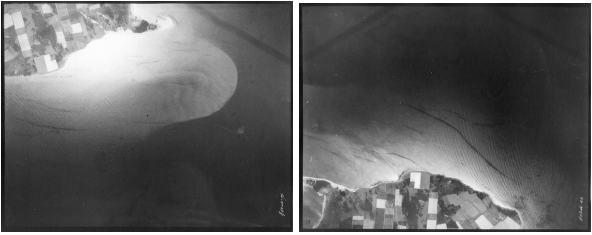
\includegraphics[width=3.0in]{figs/test}
    \caption{Example historical aerial images}
 
\end{figure}

Figure 1: Two aerial photographs overlapping the same portion of Prince Edward Island taken in 1935. The photos are not aligned (nor in the same orientation), however looking closely you can match the same parts in one image with the other. 
 
 


\section{Problem}

Estimating correspondences between images is one of the the fundamental problems in computer vision with applications ranging from large-scale 3D reconstruction to image manipulation and semantic segmentation. It is also difficult for a person to estimate the changes between the aerial images.\\       
 When we try to align the two aerial images with our eyes, first we might find an interesting point in one image that we can find in the other image. 'The island' will be the interesting feature in Figure 1.1. compare the pair image, we will have to rotate one image and shift one image a little bit to get the same orientation, and if we do this for a few more interesting points we could discover one image is bigger than the other (or more zoomed in), so we shrink one image down a little bit and continue trying to align these interesting points we have identified. Eventually we can match two images as best as we can do. Some of the interesting points may have changed slightly - like a road was repaved in a slightly different way, or a farm field is close but maybe it appears a little larger in one image and maybe the shoreline has eroded a small amount. There may not be a perfect answer but eventually you get the best alignment.That is how we approach this problem as an person. In computer vision, there are few solutions to approach this the image alignment problem.  \\
  Traditionally, correspondences consistent with a geometric model such as epipolar geometry or planer affine transformation , are computed by detecting and matching local features (such as SIFT), followed by pruning incorrect matches using local geometric constraints and robust estimation of a global geometric transformation using algorithms such as RANSAC \cite{fischler1981random}. \\
In this work we uses the convolutional neural networks(CNN) architecture that builds on the traditional approach and mimics the search for interesting points (local features) by using powerful convolutional neural networks, further a neural network can be used to find an affine transformation matrix that aligns one image with the other. Instead of the traditional algorithms such as SIFT and RANSAC. The neural network approach has a advantages over existing algorithmic approaches.\\
Speed is one of the advantages of the neural network approach. A neural network does all the learning up front, this is timely but most only be done once. When the network is trained then computing the alignment of two images is very quick. We need just apply the operations outlined by the neural network once, no training or iterations required. Compare this with an approach such as SIFT, the algorithm uses for detecting the local features from given images and followed by RANSAC\cite{fischler1981random}, the algorithm to estimate parameters from given features points.\\
Reuse is other advantages of the neural network approach. Once the NN is trained we can use it over and over again. Further to find interesting points in an image we can make use of a NN model that has already been used for image processing purposes. Finding image features is a common task and so to achieve this part of our solution we need not retrain any neural networks. We can make use of an existing and highly powerful NN to do this for us.\\
The SIFT and RANSAC solution is expensive. It has to go through the whole algorithm every time when we provide a new pairs of images, with machine learning solution, the neural networks can learn the transformation over times with labelled data, it may take longer when it is on training, but it doesn't have to start with zero knowledge every time to find the solutions, the more and well the neural network is trained, the faster and more accuracy the solution will get.\\
 A disadvantage of the neural network approach is that we are doing supervised learning. As we will outline later in the thesis, supervised learning requires a large dataset containing labelled answers. For the labelled answer means. We develop the way to harvest the aerial images and generating sub image pairs with affine transformation without the noise, and develop the labelled answer means the affine transformation matrices between the aerial image and the target images. 

\section{Interesting(Machine Learning solution)}
The rest of this paper will outline the machine learning solution that will allow us to align images.
The machine learning solution involve a dataset with paired satellite images. Taking one image and applied it with an affine transformation to generating new paired images, and label the pair images with the affine transformation.\\ 
Other part of the solution is to construct convolutional neural network to run the algorithms instead of using SIFT or RANSAC to align the images. The solution model includes feature extraction, that find the key features in given images. Feature normalization, that normalize the features that has been extracted from the images. Feature correlation that find the correlation between features. Feature Regression which will return the affine transformation between paired images.\\
\begin{figure}
\centering
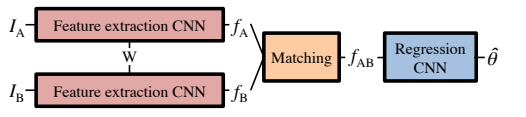
\includegraphics[width=3.0in]{figs/cnn_model}
\caption{The model that we use to produce an affine transformation matrix, $\theta$, from two source images, $I_A$ and $I_B$. \cite{Rocco17}}
\end{figure}
\begin{center}
affine  matrix = $\begin{bmatrix}
0&1&tx \\
1&0&ty
\end{bmatrix}$
\end{center}

\subsection{Feature extraction}
The feature extraction, which uses a standard CNN architecture. A CNN without fully connected layers takes an input image and produces a feature map $f \in R^{h*w*d}$, which can be interpreted as a $h * w $ dense spatial grid of d-dimensional local descriptors. For feature extraction we used the VGG-16 networks \cite{simonyan2014very}, cropped at the $ pool4 $ layer (before ReLU unit), followed by per-feature L2-normalization.The feature extraction network is duplicated and arrange in a Siamese configuration such that two input images are passed through two identical networks with share parameters.
\begin{figure}
	\begin{center}
	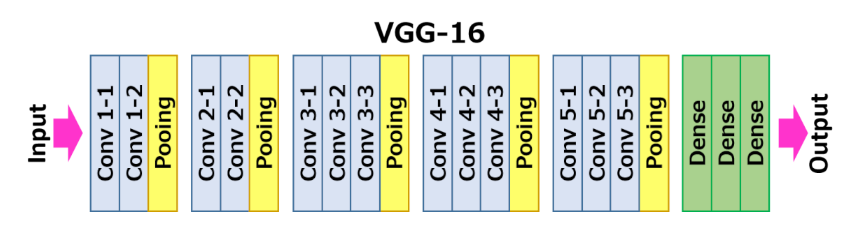
\includegraphics[width=3.0in]{figs/vgg-16}
	\caption{A listing of the layers involved in the VGG-16 Convolutional Neural Network Model.\cite{simonyan2014very}}
	\end{center}
\end{figure}
	


\section{Evaluation}
The machine learning solution apply feature extraction the neural network to replace the SIFT algorithm that find the interesting features in given images, after normalize the features, we train the feature regression neural networks with our datasets.\\
The feature regression takes in the sets of features between the two input images and predict the best parameters of the affine transformation instead of applying RANSAC which performs random sampling the regression over and over again to find the fit best parameters.\\
The machine learning algorithm takes the benefit that the machine can learn the transform of the images over times, compare to the SIFT and RANSAC that will have to start fresh whenever it gets the new images, the machine can speed by the process  training properly.\\
The goal is to evaluate the solution by comparing it against existing solutions, such as SIFT / RANSAC or manual alignment.











 % Introduction

\chapter{Background}
% affine transformation
% image alignment
%features in the images
% machine learning
% nn and cnn
% transfor learning 
% computer vision
In computer vision\cite{forsyth2002computer}, there are existing solutions to find the affine transformations\cite{mikolajczyk2004scale} between two images, mainly by using SIFT\cite{lowe2004distinctive} and RANSAC\cite{fischler1981random}. This work will focus on by using machine learning idea to do the job. This chapter will provide a background introduction to machine learning, including supervised learning, unsupervised learning. Also, the process of image alignment by using both SIFT RANSAC and machine learning.
\section{Machine Learning}
In this work we using the supervised learning to approach this problem. In supervised learning, every training data are associated with labels, in our case, the label is the affine transformation, and the data will be the images. In this section, we will provide the general description of neural network and convolutional neural network, which both are using in the model.

\section{Affine transformation}
Affine transformation\cite{svoboda2007image} take three pairs of corresponding points, which is sufficient to find the coefficients. The affine transformation includes typical geometric transformations such as rotation, translation and skewing. Affine transformation has the following properties, origin does not necessarily map to origin, lines map to line, parallel lines remain parallel after the transformation and ratios are preserved. For the translation matrix 
$\begin{pmatrix}
1&0&tx \\
0&1&ty \\
0&)&1
\end{pmatrix}$
will translate the image by $tx$ horizontally and $ty$ vertically and the rotation matrix 
$\begin{pmatrix}
\sin(\theta)&-\sin(\theta)&0 \\
\sin(\theta)&\cos(\theta)&0 \\
0&0&1
\end{pmatrix}$ will rotate the the image by $\theta$, we can take the product of the translation matrix and rotation matrix that can translate and rotate the image. 

\subsection{Neural network}
Neural networks are a popular architecture in machine learning, mainly involving input layer, hidden layers, and output layers. Each layer of a network consists of one or more neurons, each of which is connected with a weighting factor $w_{io}$ to all of the input $i$. In the simple case, the network has two inputs, as sketched in figure 2.1. 
\begin{figure}
  \centering
    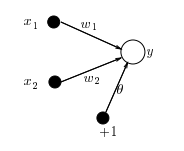
\includegraphics[width=3.0in]{figs/nn_2.1}
    \caption{Single layer network with one output and two inputs\cite{krose1993introduction}}
\end{figure}
The input of the neuron is the weighted sum of the inputs plus the bias term. The output of the network is formed by activation of the output neuron, which is some function of the inputs. 
\begin{align*}
F(y) &=  \sum_{i=1}^{2}w_ix_i+\theta
\end{align*}
There are many activation functions that we can choose, but in this work, we are mainly using the rectified linear unit, $ReLu$, a non-linear function shown in Figure 2.2.
\begin{figure}
\centering
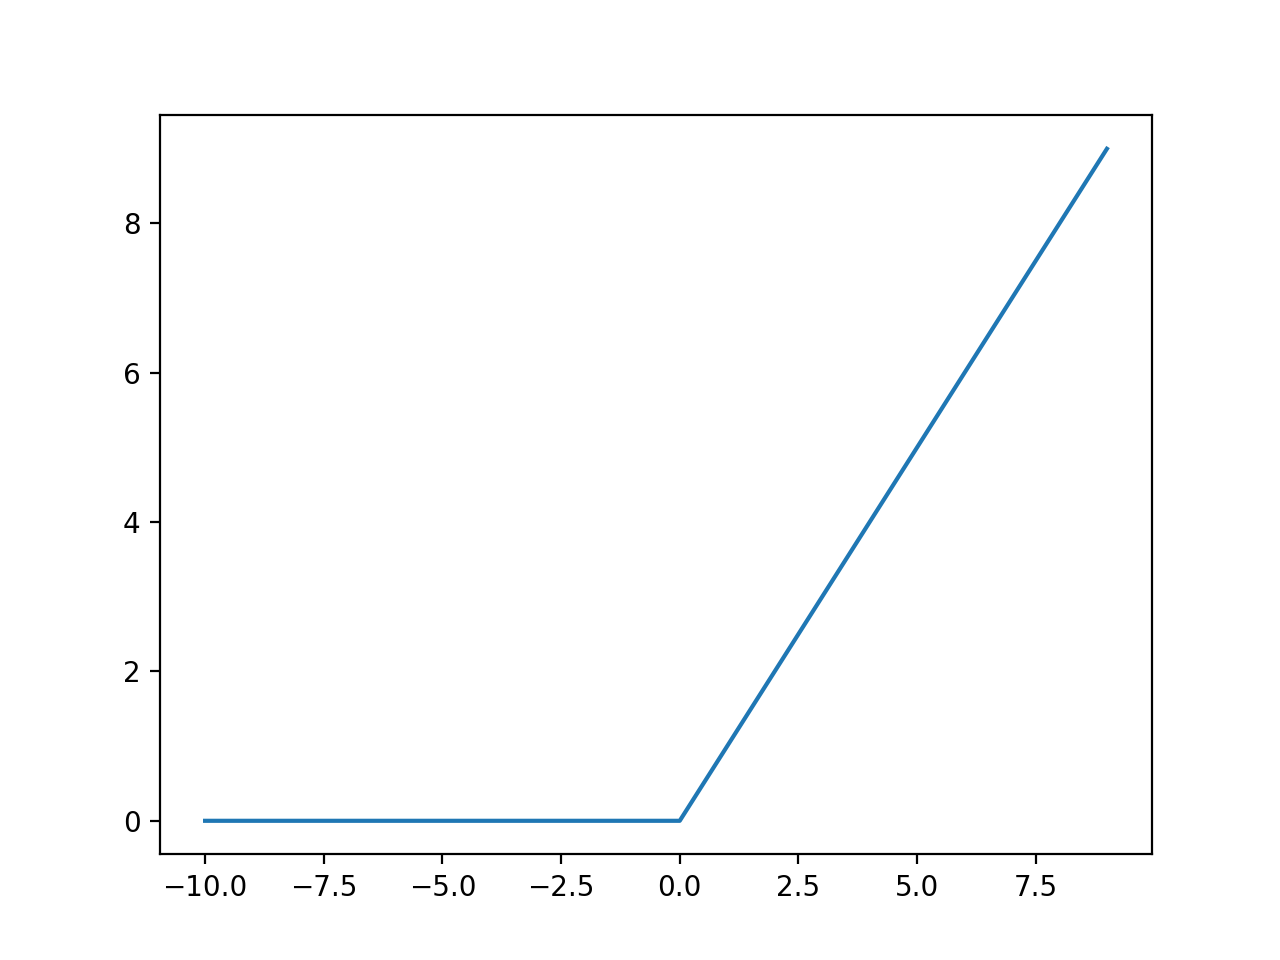
\includegraphics[width=3.0in]{figs/relu}
\caption{The Rectified Linear Unit (ReLU) activation function\cite{nair2010proceedings}}
\end{figure}
When training a network, there is two steps in training, which is forward-propagation and back-propagation. When doing forward-propagation each layer consists of units which receive their inputs from a layer directly below and send their output to units in a layer directly above the unit after the activation function. Their are no connection within a layer. After we will have some way to measure the error from the outputs, also know as $ cost\ function$. In this work we are using mean square error to measure the differences between the network prediction and the ground truth which is the parameters of affine transformation matrix in our case. After measuring the 'error', the network performs a back-propagation to adjust the weight. The trick is to apply the chain rule to find the partial derivative of the neurons. The goal of the neural network is to minimize the cost function. This is a basic neural network, also called fully connected neural network\cite{krose1993introduction}. 

\subsection{CNN(Convolutional Neural Network)}
  A convolutional neural network (CNN) is known to be good when dealing with image tasks. In this work, we are dealing with aerial photography. Using the CNN\cite{lecun1989backpropagation} is known to be efficient to dealing with image processing tasks\cite{goodfellow2016deep}. The Convolutional neural network includes a few basic concepts. First, there is a filter matrix, the purpose of the filter matrix is to detect the features in the images, and different filters may detect different features in the images.
Features can be considered like the interesting points in an image. These can include 
\begin{itemize}
\item corners where horizontal and vertical lines may meet
\item horizontal features like horizon lines
\item vertical features like edges of vertically oriented fields
\end{itemize}
Figure 2.3 shows horizontal and vertical features in an example image. When we apply the filter matrix to an image, the outcome of the image may shrink, one way to avoid this problem is applying padding to the image. There are two different types of padding, same padding or valid  padding, we can get the same size of output image after filtering by using same padding, or we can use valid padding and the size of the output image after filtering will be different than the original image. 
 
Also there is a term call 'stride' in CNN models. Stride refers to how many pixels the filter moves each time it is applied. For example if the stride is 1, then the filter is applied on every pixel. A filter starts in the upper left corner of an image. \\
\begin{figure}
  \centering
    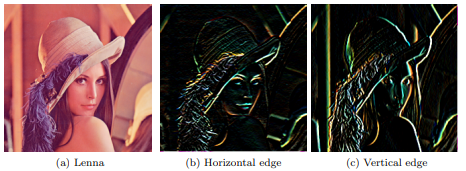
\includegraphics[width=4.0in]{figs/cnn_hv_features}
    \caption{Example image with horizontal and vertical features shown.\cite{wu2017introduction}}
\end{figure}
The convolutional layer is where the data transformation takes place. It includes many filters so that it can detect different features in the input images. After applying a convolution layer typically we apply a pooling layer. There are max pooling or average pooling, max pooling is an operation that calculates and extracts the max value in each patch of each feature map. On the other hand, average pooling operation that calculates and extracts the average value in each patch of each feature map\cite{wu2017introduction}.\\
After many repetitions of convolutional and pooling layers, we will have the fully connected layer that vectorizes all the features from the last pooling layer. This is also called a fully connected layer. \\
In the last layer, we have our loss layer, it act differently based on the loss function that we implement. Suppose $y_1$ is the corresponding label value for input $x_1$, the loss function can be used to measure how wrong is the CNN prediction $y_p$ and the $y_1$. Figure 2.4 shows the general architecture of a CNN model.



\begin{figure}
  \centering
    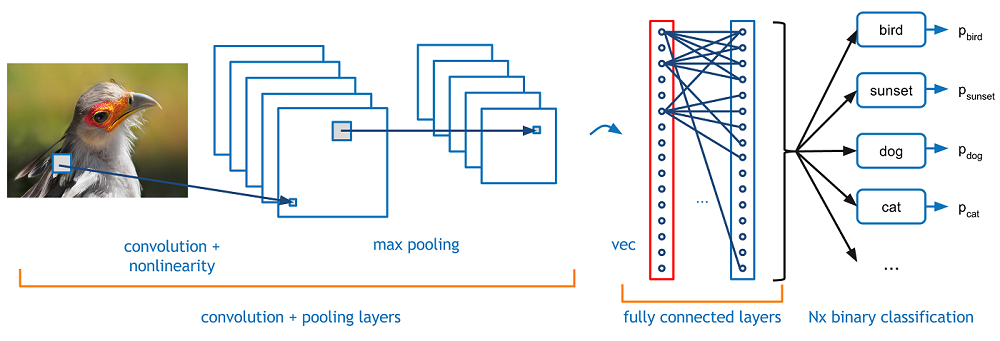
\includegraphics[width=4.5in]{figs/cnn_arch}
    \caption{The architecture of a CNN\cite{cnn}}
\end{figure}

\subsection{Transfer learning}
Transfer learning\cite{pratt1997second} can be very useful with certain machine learning or data mining model. Transfer learning allows us to use the knowledge within a neural network that has already been trained and apply that knowledge to help solve a new task. That means we can find a neural network that is has been trained to do some task, and we strip of the last few layers in the pre-trained neural network and add own customized layers after that, so that when we train the neural network we only need to train the new layers that we added while retaining the knowledge of the other layers.\\
The problem of building and training a model from scratch is that sometimes it is too hard or is impossible to collect enough data for the model, or it takes too much resources to train and build the model from scratch. By using transfer learning, we may avoid these expenses. Transfer learning can be applied to different machine learning problems like regression, classification or clustering.\\
In transfer learning, we find a pre-trained machine learning model and we only keep the part that we need to keep in the model, and we add some new layers after. We only need to train the layers that come after the original model, which can save data and time. Figure 2.5 shows briefly how transfer learning works.

\begin{figure}
  \centering
    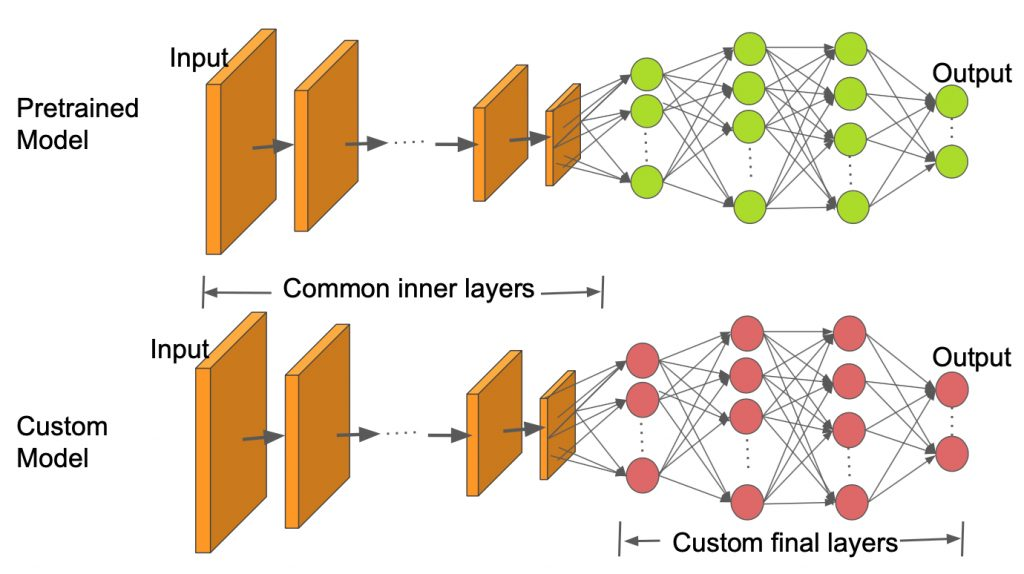
\includegraphics[width=3.0in]{figs/transfer_learning}
    \caption{A pre-trained model (above) has the last layers (green) removed and replaced so that the model may be reused for a new task (below). This process is called Transfer Learning.\citep{TL}}
\end{figure}


\section{SIFT and RANSAC}

One of the traditional solution for finding an affine transformation between two images is by using SIFT and RANSAC algorithms. The Scale Invariant Feature Transform(SIFT) is capable of finding the interesting features in a image even if the image is scaled or rotated. \cite{lowe1999object}\\
\begin{figure}
	\centering
	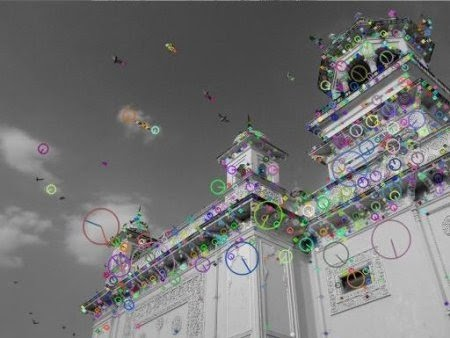
\includegraphics[width=3.0in]{figs/sift}
    \caption{Example of the SIFT algorithm finding interest points (features) in an image.\cite{sift_cv}}
\end{figure}

The Random Sample Consensus(RANSAC) estimates the parameters of a model by random sample of observed data and comes up with the best parameters that fit most of the data. After we have the found correspondences between features in two images we can generate the transformation matrix to align those two pictures.
\begin{figure}
	\centering
	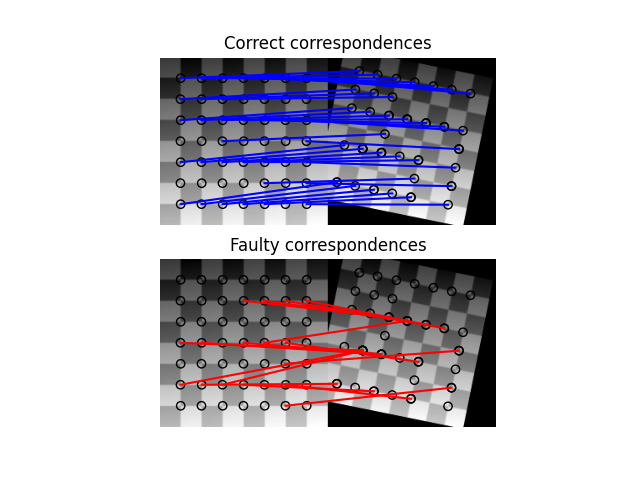
\includegraphics[width=3.0in]{figs/ransac_correct}
    \caption{Example of the RANSAC algorithm finding correspondences between two images.\cite{ransac_ski}}
\end{figure}

\section{Image Alignment}
This section will provide a high level introduction to image alignment and stitching. Image alignment involves many algorithms that work together so that the computer can align multiple images and stitch them together. Image alignment involves:
\begin{itemize}
\item finding common features between two images
\item matching the common features
\item generating the transformation between the images so that we can align them together.
\end{itemize}
 
For given two images, the first step is to find the common features between those images. Traditionally this may be done using SIFT \cite{lowe2004distinctive}. SIFT became a popular tool for finding common features in images between it is robust to handle images that vary in orientation, zoom and illumination. In simple terms SIFT can handle rotations, shifts and different colors in images.\\
Second, after we have found features in the images we need to find which features in one image match to which features in the other image. We can use RANSAC\cite{fischler1981random} for this goal. RANSAC will allow us to estimate the image transformation parameters that will align a number of features in one image with a set of features in another image. The following indented section follows from Brown and Lowe \cite{brown2007automatic} in their paper that outlines who to perform image stitching using RANSAC.\\
\begin{quote}
We denote the features that overlap in an image as $n_f$ and number of inlier $ n_i$. The trial result of image matching has one of two outcomes: $ m \in \{0,1\}$, and also for each trial for the feature matching $f^(i) \in \{0,1\}$ also only has binary outcomes, we assume it to be independent Bernoulli, so the number of inliers can be fit into Binomial distribution:\\
\begin{align*}
	p(f^{1:n_f} | m=1) = B(n_i;n_f,p1)\\
	p(f^{1:n_f} | m=0) = B(n_i;n_f,p0)
\end{align*}
Where the Binomial distribution is define as below:
\begin{align*}
	B(x;n, p) = \binom{n}{x} \cdot p^x(1-p)^{n-x}
\end{align*}
We can choose the value of $p_1 =0.6$ and value of $p_0 =0.1$, and we can applying  Bayes' Rule to find out if the images are matching:
\begin{align*}
p(m=1|f^{1:n_f}) = \frac{p(f^{1:n_f} | m=1) \cdot p(m=1)}{p(f^{1:n_f})}
\end{align*}
that give us the probability of if the image is matching base on the probability of the feature matching in the image. In Figure 2.8, shows the outcome of an image alignment and stitching example using aerial photographs.
\end{quote}



   

\begin{figure}
  \centering
    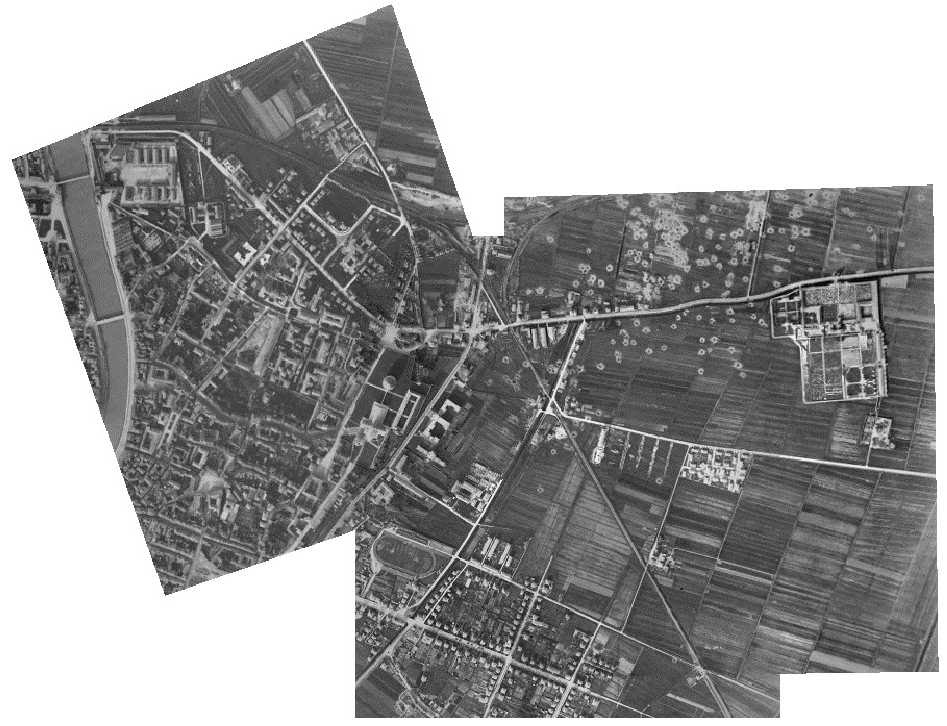
\includegraphics[width=3.0in]{figs/img_alignment}
    \caption{Aerial image alignment and stitching from three aerial photographs containing overlapping data.}
\end{figure}


 % Background Theory 

\chapter{Dataset}
In order to train the parameters of the geometric matching CNN model, it is necessary to design the appropriate dataset architecture with suitable training data. The dataset includes two parts. The first part is the images that we use to train the model, this includes both source images and target images. The target image is generated from the source image by an affine transformation. The second part of our training data is the transformation between the source image and target image, the affine transformation, which serve as the label during the training process. We will address the dataset in this chapter.
\section{API}
We use the $google\ map\ static\ api $ to get our high quality aerial images of Prince Edward Island. We select the aerial images by providing the longitude and latitude values to access an image location. The API also has ability to choose the size of an image, also the center of the image. 

\begin{figure}
 \centering
    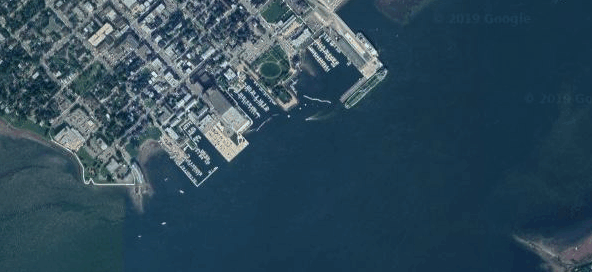
\includegraphics[width=3.0in]{figs/charlottetown}
    \caption{46.2382° N, 63.1311° W, Charlottetown}
\end{figure}


\section{Image}

For training our neural network, an image containing a black bar with unknown data is of no use, we must know what data is supposed to be where the black bar is. In other words we need to know what the aerial photograph should look like if taken from that vantage point. To solve this issue we have come up with the following strategy.\\
  We take a big picture and crop the center square of this big picture. Call this center square the \textit{source image}. Now apply an affine transformation (a rotation or shift or both) to the center square in the big picture. This affine transformation will move the square to some new location and orientation in the big picture. Cropping the big picture using this new square at its new location gives our \textit{target image}. See Figure 3.3. We have that the source image * transformation = target image and there is now no unknown data (no black bars). The source and target images are the inputs to our CNN model. While the transformation matrix serves as the label for supervised training.
\begin{figure}
 \centering
    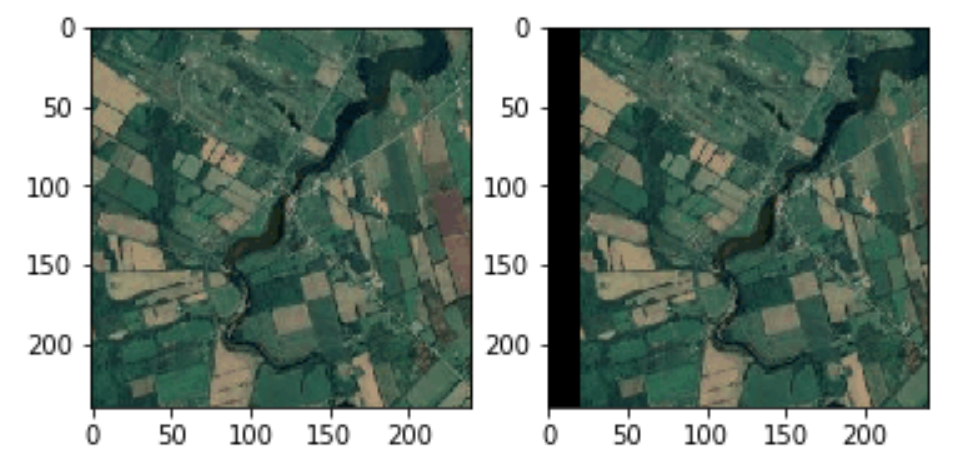
\includegraphics[width=4.0in]{figs/affine_noise}
    \caption{Applying an affine transformation to the image at left, yields the transformed image at right. Notice the black bar on the left side of the transformed image.}
\end{figure}

\section{Training data}
The training dataset includes the source images and the target images. We generated the source images from the API from the previous section, generated the target images by applying transformations to source images.\\
  From each source image, we generate 195 target images by applying a variety of different affine transformations to the source image. Each transformation yields a different target image. We applying the affine transformation that can shift the image first, thus generating the different $tx\ ty$ value in an affine matrix $\begin{pmatrix}
 1 & 0 & tx \\
 0 & 1 & ty
 \end{pmatrix}$, which can shift a image up/down and left/right. For each of the shifted image, we can rotate the images by $ 90,\ 180,\ 270$ degrees, respectively thus generating more target images. We do all of our image manipulations to build the dataset of images using opencv\cite{bradski2000opencv}. Thus for each source image, we can shift the image to obtain a new image, or rotate it, or we can applying both shift and rotation to generate many target images. The architecture of the dataset involve the source image, target image and the  labels. 
 The source images and target images are passed to the CNN model at same time, since we are doing the supervised learning, we also need labels associated with the inputs. The labels are the affine transformation that aligns the source image over top of the target image. If we were generating shift images and rotation images, we will multiple the shift matrix and rotation matrix together. Thus we have a training set containing source images, target images and affine transformations that align a source image with a given target image, this is all the requirements for our supervised machine learning task. We generate 10,000 image pairs including corresponding affine transformation matrices to facilitate our supervised training task. An example of a source and target image are shown in Figure 3.3.

 
\begin{figure}
\centering
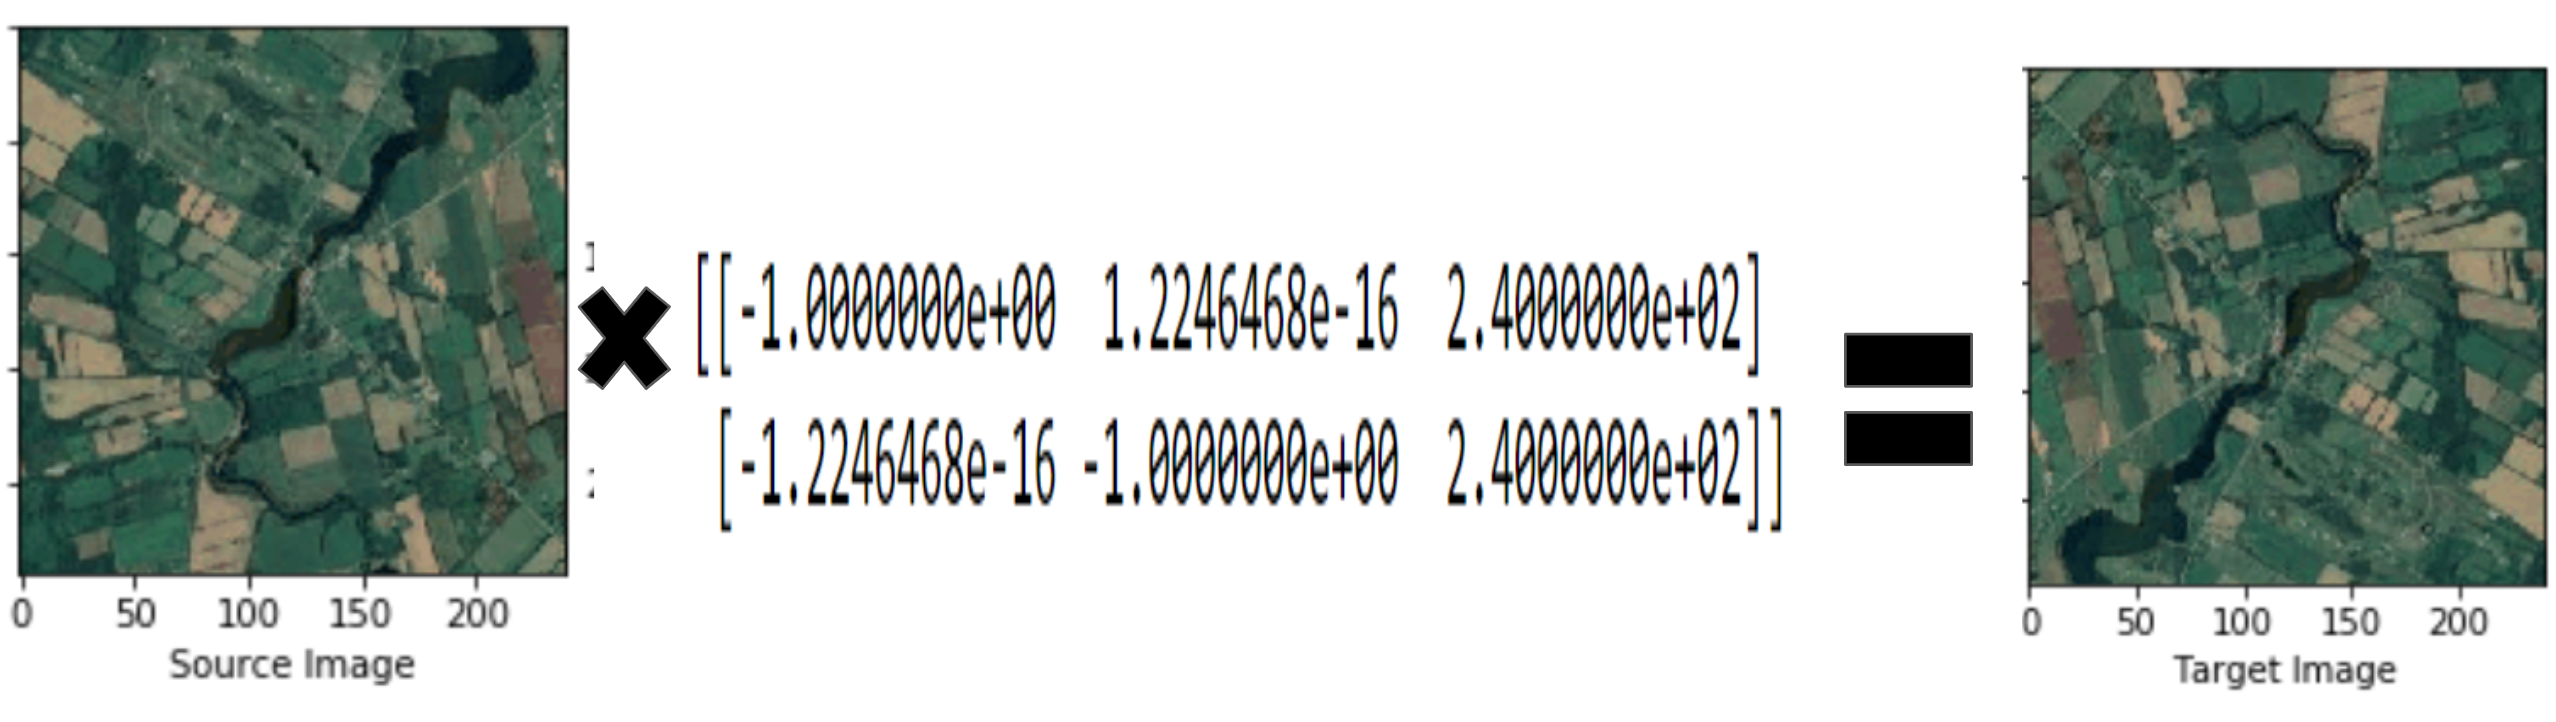
\includegraphics[width = 4.5in]{figs/source_target}
\caption{training image pair}
\end{figure}

\section{CSV File}
In order to access the images and the transformation from the code, we need to be able to store the data in some manner. We choose to store the data in a csv file containing the following information: 
\begin{itemize}
\item path to the source images
\item path to the transform(target) images
\item the affine transformations associated with the source and target images.
\end{itemize}
The affine transformation are labelled as \verb+A00 A01 tx A10 A11 ty+,\\
where A00 gives the entry in the top left corner (0,0) of the affine transformation matrix. The csv files will have at least eight columns includes images paths followed by six columns representing each index in the affine transformation matrix with the order given above.

\section{Format}
In the Feature Extraction part of the CNN model, we are using a pre-trained neural network VGG-16 \cite{simonyan2014very}. The default input images are $ 244 * 244 $, any size changes of the input may change the result of the output. The affine transformations  The VGG16 architecture are shown in Figure 3.4. 
\begin{figure}
 \centering
    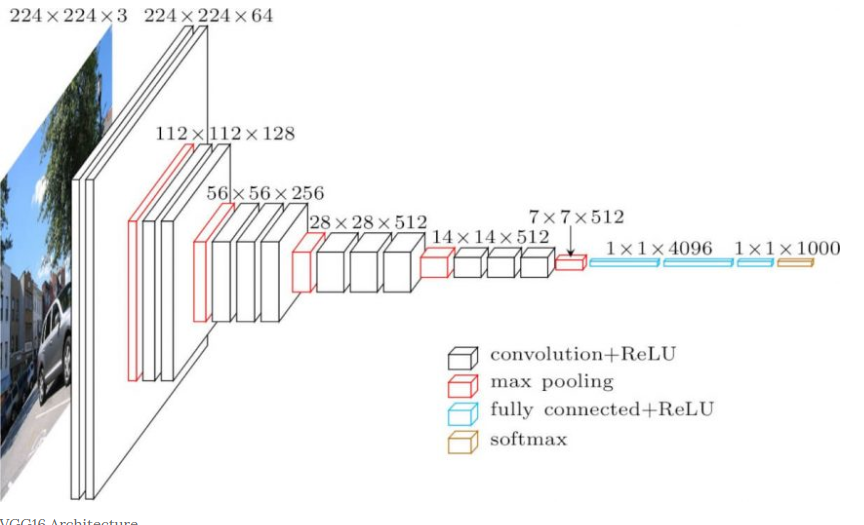
\includegraphics[width=3.0in]{figs/vgg16_architecture}
    \caption{VGG16 Architecture\cite{vgg_arch}}
\end{figure}

  VGG-16 is a convolutional neural network that has already been trained to solve complex image classification tasks. This means it can identify what is in an image (classification). We are not concerned with what is in an image, however as part of VGG-16's training it learns lots of information about images which is then contained within its layers. This information can be thought of as the features that help determine what an image is. We remove the last layers of the VGG-16 network and use the raw data within the layers VGG-16 as our image features. In other words this replaces the traditional task of SIFT to find those interesting portions of an image. These interesting portions of an image are what we call features. This process is outlined in Chapter 2, and is known as transfer learning. We use a pre-trained network and apply its knowledge to help with a different task. In our case we are concerned with finding features within an image (feature extraction), something that VGG-16 is already good at. % Experimental Setup

\chapter{The Model}
This chapter explains the the paper "Convolutional neural network architecture for geometric matching\citep{Rocco17}" from Rocco, I. and Arandjelovi\'c, R. and Sivic, J. This paper gives a solution for the transformation between two images such as an affine transformation or thin-plate spline transformation, and estimating the parameters. This work gives the neural network model that we will build to try and solve our similar task involving the alignment of aerial images.

\section{Model}
In the geometric matching project\citep{Rocco17}, they propose a convolutional neural network architecture for geometric matching that includes three main components:
\begin{itemize}
\item CNN that mimics the standard steps of feature extraction.
\item the feature matching. 
\item simultaneous inlier detection and model parameter estimation.
\end{itemize}
  In a broad sense the process to align images with neural networks involves two approaches, a transfer learning approach to extract features, and a supervised learning approach to determine the affine transformation that will align features in paired images. Features can be extracted using a pre-trained neural network such as ResNet101\cite{dai2016r} or VGG-16\cite{simonyan2014very}. These are large networks originally designed to classify massive image datasets. We use the pre-trained model VGG 16 to do feature extraction. We crop off the last pooling layer of this network (before the ReLU activation) and perform L2 normalization. This is our transfer learning approach that uses the existing knowledge of images in the VGG 16 model. Our work here follows the work of Rocco\citep{Rocco17}. Feature regression (also known as finding the best alignment between the features of two images) is the part where supervised machine learning and a labelled dataset such as that described in Chapter 3 is required. The whole model is shown in Figure 4.1.

\begin{figure}
\centering
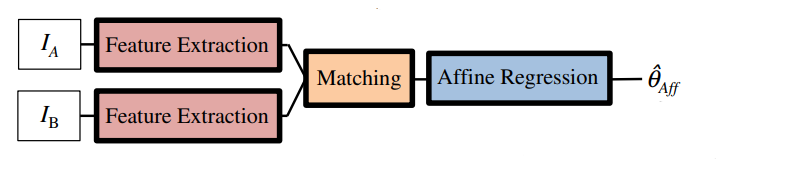
\includegraphics[width = 3.0in]{figs/cnn_model_aff}
\caption{CNN Model showing 3 steps in our process to arrive at $\theta$, which represents the transformation that can be applied to image $I_A$ to best align it with image $I_B$ (the inputs to the model).\cite{Rocco17}}
\end{figure}
\section{Input and output}
Refer to Figure 4.1, the input will be the two images that are passed into the model simultaneously (a source image and a target image). It should be noted that the images must have some overlap or commonalities, otherwise it makes no sense on how to align them. See Figure 4.2. The images go through the feature extraction CNN which is a pre-train neural network (VGG-16$pool4$) and return all the features that the network found in the input images. Note that Figure 4.2, only shows a few example features, simulated with red dots for clarity of understanding only.\\
  After feature extraction, we follow a L2-normalization to normalize all the features, and return the normalize features set for each image. After that we find the correlation between the normalized images. Feature correlation takes in two sets of the normalize features and returns a correlation tensor containing the correlation between each feature sets. We normalize the correlation in the same way that we normalize the extracted features.\\
  Estimating the parameters of the affine matrix is called feature regression, it is a CNN model that we train with our dataset, which takes in the normalized correlation sets and returns the affine matrix, denoted by $\theta$.
 
\begin{figure}
\centering
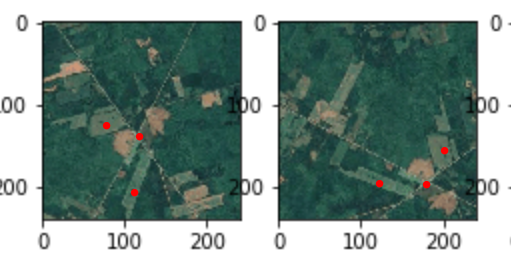
\includegraphics[width = 3.0in]{figs/data_example}
\caption{Two example images with red dots showing common points between the images. These images may be used as input to our model.}
\end{figure}
\section{Required label}
In order for the model to learn the affine transformation matrix, we need to pass the real matrix values to the model during the training phase, the affine transformation matrix  has six parameters, we put the matrix parameters in a csv file where each row of the file contains the following: A00, A01, tx, A10, A11, ty and their corresponding position in the affine transformation matrix given below:

$\begin{bmatrix}
A00& A01& tx \\
A10& A1& ty
\end{bmatrix}$\\
Rocco et al. \cite{Rocco18}, outline two ways to pass paired images and their corresponding affine transformation matrix into the model. One way is to only pass the source image path, and the parameter labels, which they call synth-dataset\cite{cnngeometric_pytorch}. The single image is altered to produce two images synthetically. The other way is passing the path to both a source and target image with labels and a bounding box giving the area in the image that is shared between the source and target. This is called a coupled-dataset \cite{cnngeometric_pytorch}, the coupled-dataset is what our work uses when we serve the training data to the model. 

\section{Learning}
In the paper\citep{Rocco17}, off which we base this project, the full model can be thought of as a pipeline (see Figure 4.3), the inputs to the pipeline are the source and target images. First step is to find features in the images, next we correlate the features and finally we determine the affine transformation aligning those features. This is done as part of a learning process, meaning the outputs are the raw values that make up the affine transformation matrix. Our goal is to adjust the neural network so that the outputs of the network match our labels, the ground truth affine transformations we already determined when we built the dataset.\\
  It should be noted that the goal of Rocco et al. \cite{Rocco17} differs from our own goal. See Figures 4.4,4.5 4.6 which show some of their results. The focus is on aligning certain aspects of an image, such as a car, or duck for instance.\\
  In our work we focus only on aerial photography. We assume that the photographs are taken from air planes with a camera pointing down and so viewing angles are less of a concern for us. We are only concerned with finding the affine transformation matrix between the two images. In some ways our task may be considered easier than Rocco et. al, because we do not concern ourselves with twists and deformations (such as deforming the duck in Figure 4.4, to match the target duck. However, our task may also be considered more difficult since we have images sometimes have a uniform appearance. For example an image with green fields. Finding features in such images could be quite challenging since the image looks the same in many parts.
\begin{figure}
\centering
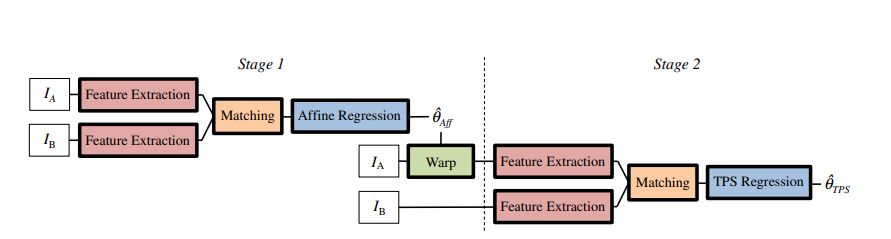
\includegraphics[width = 3.0in]{figs/full_arch}
\caption{The full model use by Rocco et, al.\cite{cnngeometric_pytorch}. Their full model was intended to warp and twist portions of an image for best alignment. We do not use the full model, as we assume aerial photographs to be roughly taken from the same relative position to the earth. In other words we assume the plane flies horizontal with a camera pointing down.}
\end{figure}
 The model learns how to apply affine transformation by finding the the key features in the source image and the target image, and find the transformations between the key features, apply each transformation to the source images and translate the images, finally, the model will apply affine transformation to the image, see Figure \ref{fig:4.3} shows how the source will translate corresponding on affine transformation. Also, the Figure \ref{fig: 4.4} marks the key points in the source image and the target image, also the translated images.\\ 
\begin{figure}
\centering
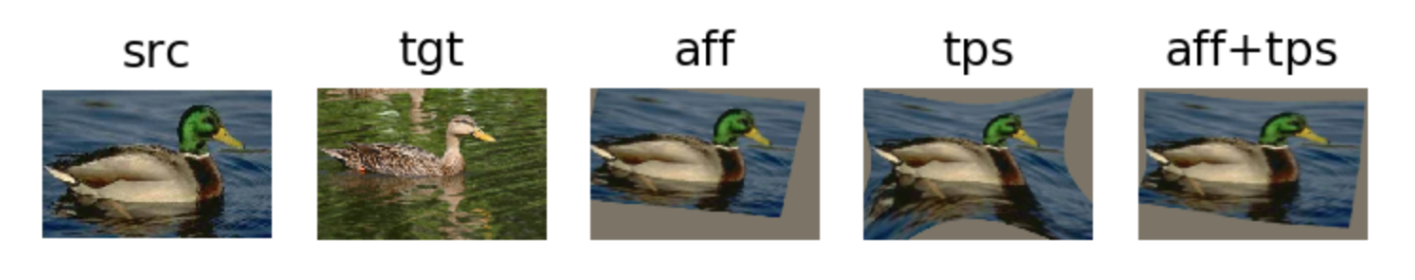
\includegraphics[width = 4.0in]{figs/aff_tps}
\caption{In the demonstration by Rocco et al\cite{Rocco17}, they show the alignment of two images containing similar ducks}
\end{figure}
The Figure 4.5 demonstrations of alignment between images that share characteristics. Note that a bounding box is used to single out the parts of the image that are in common. That the images are taking from "Qualitative results on the Tokyo Time Machine dataset\citep{Rocco18}".\\
\begin{figure}
\centering
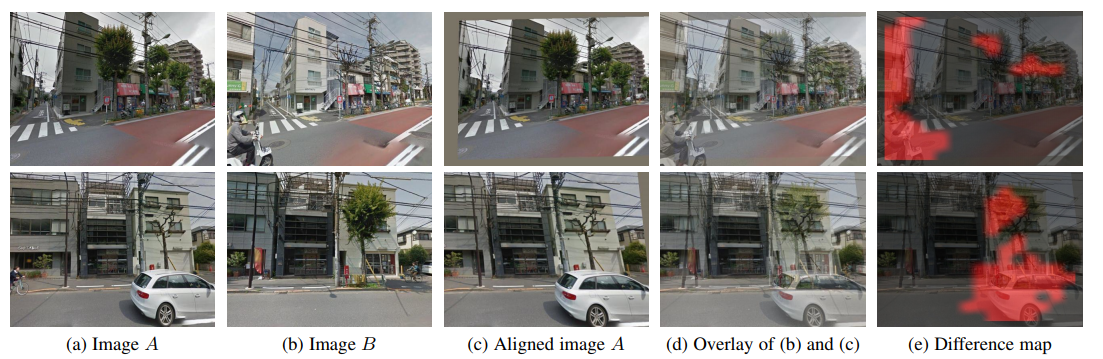
\includegraphics[width = 4.0in]{figs/overlap}
\caption{In the demonstration by Rocco et al\cite{Rocco18}, they show the finding the overlap between images}
\end{figure}
  The Figure 4.6 outline the boundary box that single out the key feature between images from the paper\citep{Rocco17}.
\begin{figure}
\centering
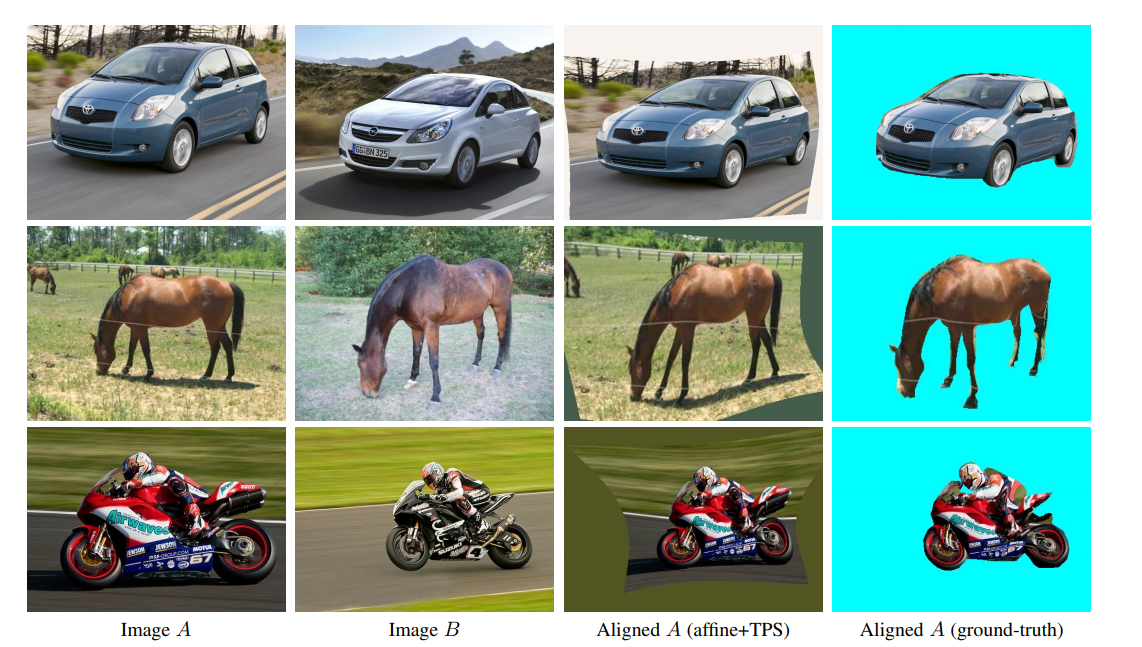
\includegraphics[width = 4.0in]{figs/bound_box}
\caption{In the demonstration by Rocco et al\cite{Rocco18}, they show the bounding box that single out the key feature between images}
\end{figure}
 

\begin{figure}
\centering
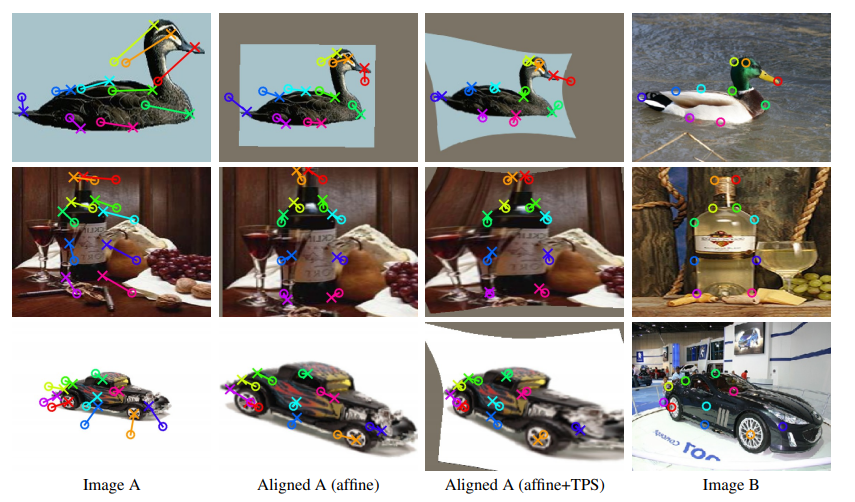
\includegraphics[width = 4.0in]{figs/keypoint_examples}
\caption{Model demo \cite{cnngeometric_pytorch}}
\end{figure}
  We are using the first part of the model and train it with our own aerial dataset and the model will learn how to find the affine transformation parameters between two aerial images. The model will concat with two neural network, the first part is a pre-trained neural network VGG16 that is used for feature extraction. The images each pass through the same network (our pretrained VGG 16 model) to extract image features. Recall the image features are computer distinguishable characteristics in the image, such as color changes, lines, corners, and various local pixel differences that respond to the convolutional filters. This follow by the layer matches those features, the matching layer use a correlation layer followed by normalization. First, all pairs of similarities
between descriptors are computed in the correlation layer. Secondly, similarity scores are processed and normalized such that ambiguous matches are strongly down-weighted\cite{Rocco17}.
The last part of the model is the regression network, which directly estimates parameters of the geometric transformation relating the two input images.\\
  As we mentioned previously a neural network requires a cost function to facilitate training. In other words a measure of how wrong the network is. For this task we use mean squared error \cite{mse}. Mean squared error gives a measure of the average squared difference between the estimated values and the ground truth value. In our case MSE is calculated between the individual values that make up the affine transformation matrix that the model produces and the individual values that make up the affine transformation matrix in our ground truth.\\
  There are other cost functions that may be used. For example in Rocco et, al. \cite{Rocco17} they also propose a cost function that applies the generated transformation to the source image and compares pixels in the newly generated image and the ground truth applied to the source image. We discuss our cost function in further details in the next chapter.
 % Experiment 1

\chapter{Results}
In order to train the CNN model, we need to select the appropriate loss function and design suitable training data. We address these two important points in this chapter and provide the implementation detail.\\
  This chapter will also outline the implement detail of the model, the demo output of the model and also show the output by using SIFT\citep{lowe2004distinctive} and RANSCAC\citep{fischler1981random} algorithm. We also present some observations and discussion surround the presented results. \\
  


\section{Training}
This section gives the implementation detail, includes the implementation of the training data and the implementation of the neural network. 

\subsection{Training data}
The model requires fully supervised training data includes image pairs and known affine transformation between images. Training a CNN requires a lot of data, we couldn't find the public dataset that has paired aerial images and associate with the affine transformation, so we created our own dataset.\\
  The aerial images are harvested through the google static map api, we generated more than 10,000 image pairs and labels and kept them into a CSV file to serve to the model. The images all have the same size(240*240)
\subsection{Loss function}
  We are doing supervised learning, the training data are the paired images and the desired output in the form of the parameters $\theta_{AF}$ of the ground-truth affine transformation. The loss function $L$ is used to compare the estimate affine transformation $\theta$ and the ground-truth affine transformation $\theta_{AF}$. The goal is to minimize the loss function by using backpropagation and Gradient Descent.\\
  There are many loss functions, we choose to use Mean Square Error(MSE) as the loss function for the model. MSE takes the square of the difference between the $\theta$ and the $\theta_{AF}$, sum all the difference for all the input and divide it by the number of the input $N$.
\begin{align*}
MSE = \frac{1}{N}\sum_{i=1}^{N}{(\theta - \theta_{AF})}^2
\end{align*}
  We can compute the the gradient of the loss function with respect to the estimates 
  $\frac{\partial L}{\partial \theta}$, the gradient of the loss function with respect respect to the transformation parameters, needed to perform backpropagation in order the neural network update so that it can learn. 

\subsection{Implement detail}
  We choose to use the Pytorch\cite{pytorch} library to implement the model. PyTorch is a machine learning and neural network library that facilitates building and training machine learning models. In PyTorch back propagation equations and implementations for common loss functions such as MSE are already implemented. We use those implementations. We implement the model from Rocco, I\citep{Rocco18}, so we have the same learning rate$10^-3$, and train the network using the Adam optimizer\cite{kingma2014adam} and batch size of 16. \\

\section{Experiment result}
This section will gives some examples of the our results, which focus on aerial photographs of various points over PEI. We present results showing the alignment between our machine learning approach, and the SIFT and RANSAC approach and finally we will do a manual alignment and show those results.

\subsection{Machine learning results}
We are using the model that is trained by Rocco,I\cite{Rocco18} to test the result of our aerial images. 
The aerial images are taken from our dataset and contain only those images with translations. The translations range between 0 and 120 pixels in either of the x or y directions. Recall that our images are 240 pixels total. So the translations may be up to half the image in either direction.\\
  In the image alignment process, we need to find the key features in the given images, the machine learning approach replace that by using pre-trained CNN, and we will estimate the parameters of the affine transformation by using another CNN. 
  We will compare the results of the of the estimate affine transformation by the ground truth affine transformation.
  The Figure 5.1 shows the results of the the machine learning affine transformation result and the ground-truth affine transformation. The ground truth affine transformation for this is: (put this into a matrix or table:[[1, 0, 20] [0, 1, -20] [0, 0, 1]]. After normalization this becomes: [[1, 0, -0.1639 ] [0, 1, 0.1639 ] [0, 0, 1 ]] while our machine learning algorithm produces an estimated normalized affine transformation of : [[0.9916, 0.0089, -0.1623] [-0.0268, 0.9917, 0.1670] [0, 0, 1]]. While visually the ground truth and machine learning estimate look very similar, they are also similar in terms of error, with a MSE for the normalized affine transformation matrices of 0.0002.\\
\begin{figure}
\centering
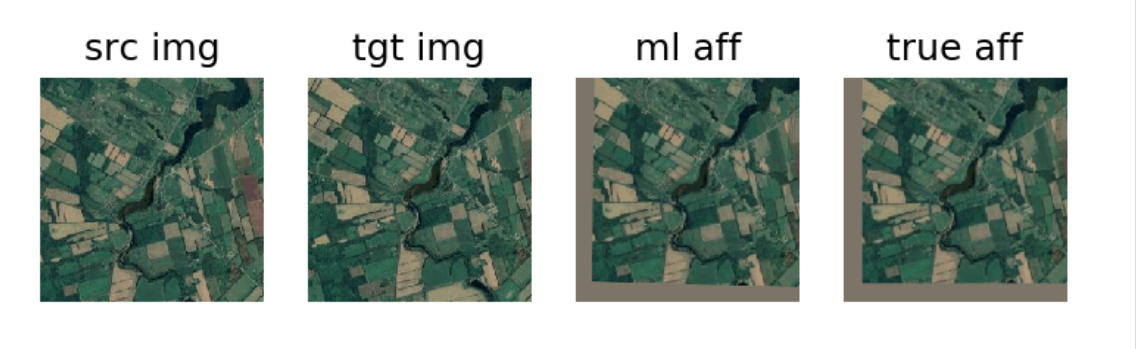
\includegraphics[width = 5.0in]{figs/ml_affine_similar}
\caption{The source (src) and target (tgt) images at left are sent into the machine learning model to produce the affine transformation that may be applied to the source and produce the target. This is shown in the image under heading ml aff. Finally the actual ground truth affine transformation applied to the source image is shown. The ground truth affine transformation represents a shift of 20 pixels to the right and 20 pixels up.}
\end{figure}
  Similar strong results can be seen in Figure 5.2. However even visually in Figure 5.2 we can start to see that the machine learning algorithm contains some errors. Most notably, visually, the image is translated to roughly the correct spot but it has been warped and rotated slightly. The ground truth affine transformation is [[1, 0, 40] [0, 1, 40] [0, 0, 1]]. After normalization this becomes: [[1, 0, -0.3279] [0, 1, -0.3279] [0, 0, 1]] compare to our machine learning algorithm produces an estimated normalized affine transformation of : [[1.0253, -0.0262, -0.2504] [0.0604, 0.9509, -0.2714] [0, 0, 1]],  with a MSE for the normalized affine transformation matrices of 0.0028.\\
\begin{figure}
\centering
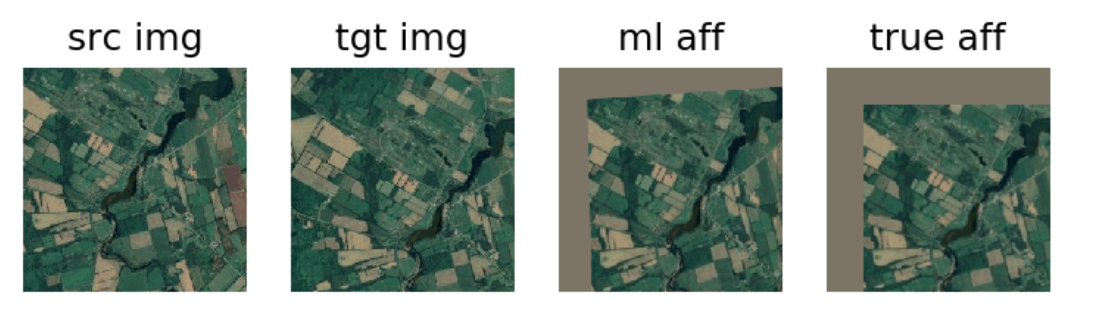
\includegraphics[width = 5.0in]{figs/40_right_40_down}
\caption{Source and Target Images sent into our model produce the ml aff image. Shown last is the actual ground truth solution. The affine transformation for this image pair is a 40 pixel shift right and 40 pixel shift down. Visually our model produces a pleasing result.}
\end{figure}
  In Figure 5.3 we start to see where the model fails. Translations beyond 60 pixels (this figure has a 60 pixel translation to the right and 60 pixels down. The affine transformation for the ground truth and our machine learning estimate are [1, 0, -0.4918] [0, 1, -0.4918] [0, 0, 1]] and [[ 0.8462, -0.0698, -0.0376] [0.0479,  0.8448, -0.0681] [0, 0, 1]] which represents a MSE of 0.0735.
\begin{figure}
\centering
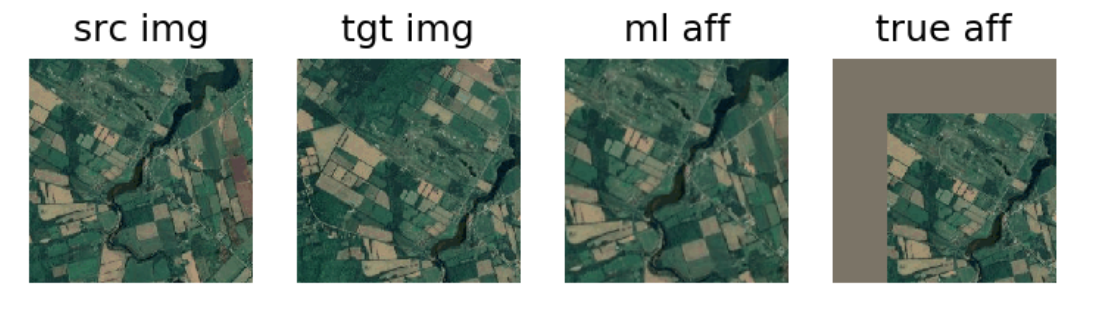
\includegraphics[width = 5.0in]{figs/60_right_60_down}
\caption{Source and Target Images sent into our model produce the ml aff image. Shown last is the actual ground truth solution. The affine transformation for this image pair is a 60 pixel shift right and 60 pixel shift down.}
\end{figure}


\subsection{SIFT and RANSAC}
  The SIFT\cite{lowe2004distinctive} and RANSAC\cite{fischler1981random} algorithms can be uses to find the affine transformation between the source image and the target images. Chapter 2 gives an introductions of SIFT and RANSAC algorithm, we can use SIFT to detect key points in the images, and uses RANSAC to estimate parameters of the transformation.\\
  This section shows a few example images and their affine transformations determined by SIFT and RANSAC. We use the same input images as we used in the machine learning approach, the images are just randomly selected from our dataset representing different degrees of translations.\\
   Figures 5.4, 5.5 and 5.6 show the results when using the SIFT and RANSAC approach. Visually, the method is clearly strong and the alignment is pleasing. The color difference between the unknown portion (black versus grey) left behind after the translation is just an artifact of the display library used to display the images.
   
\begin{figure}
\centering
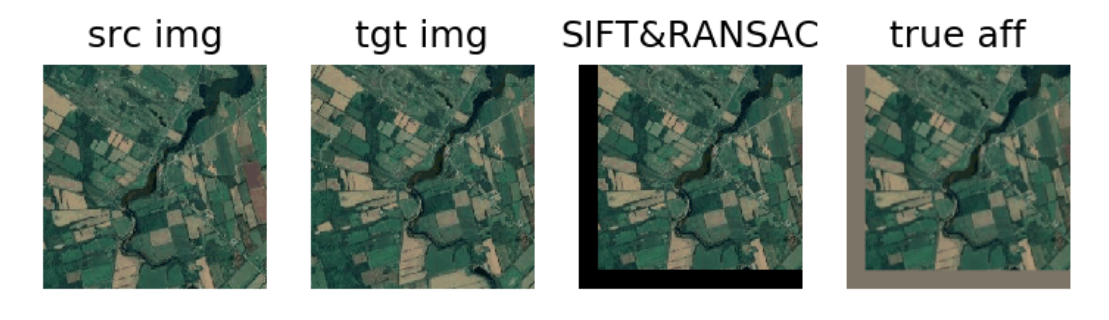
\includegraphics[width = 5.0in]{figs/sift_20r_20up}
\caption{Applying SIFT and RANSAC to the source(src) and target(tgt) images produce the SIFT and RANSAC image are shown. While the ground truth is shown at far right. The ground truth normalized affine transformation matrix is [[1, 0, -0.1639 ] [0, 1, 0.1639] [0, 0, 1]] while with SIFT and RANSAC with normalization we get an affine transformation matrix of [[0.9999, 0.0, -0.1666] [0.0, 0.999, 0.1667] [0, 0, 1]]}
\end{figure}

  
\begin{figure}
\centering
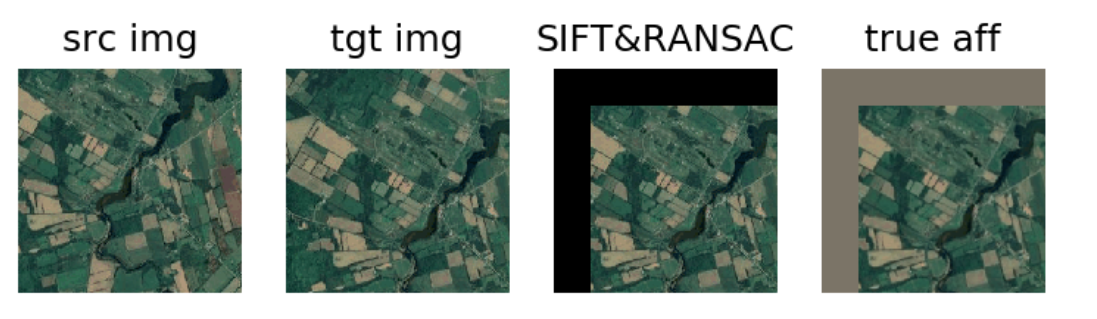
\includegraphics[width = 5.0in]{figs/sift_40down_40right}
\caption{Applying SIFT and RANSAC to the source(src) and target(tgt) images produce the SIFT and RANSAC image are shown. While the ground truth is shown at far right. The ground truth normalized affine transformation matrix is [[1, 0, -0.3279 ] [0, 1, -0.3279] [0, 0, 1]] while with SIFT and RANSAC with normalization we get an affine transformation matrix of [[0.9999, 0.0, -0.3333] [0.0, 0.999, -0.3333] [0, 0, 1]]}
\end{figure}


\begin{figure}
\centering
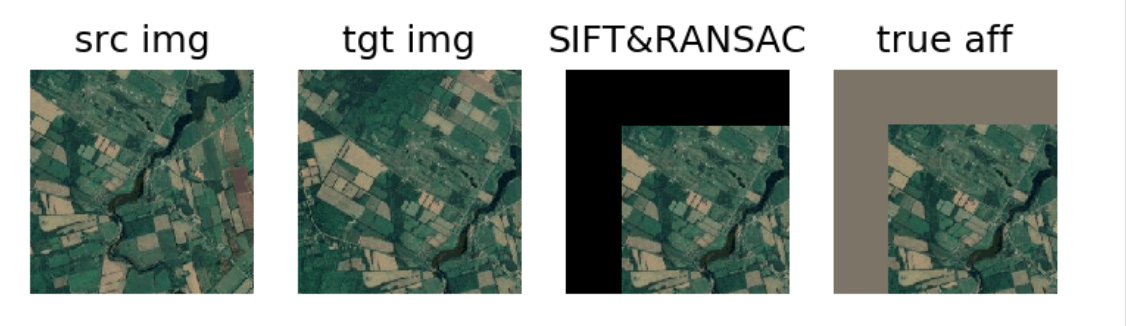
\includegraphics[width = 5.0in]{figs/sift_60down_60right}
\caption{Applying SIFT and RANSAC to the source(src) and target(tgt) images produce the SIFT and RANSAC image are shown. While the ground truth is shown at far right. The ground truth normalized affine transformation matrix is [[1, 0, -0.4918 ] [0, 1, -0.4918] [0, 0, 1]] while with SIFT and RANSAC with normalization we get an affine transformation matrix of [[0.9999, 0.0, -0.4999] [0.0, 0.999, -0.4999] [0, 0, 1]]}
\end{figure}


\subsection{Manual}
We can manually compute an affine transformation matrix by manually identifying the same points in each of the source and target images. We build a small program that produces an affine transformation after we click on three points in the source image and then the same three points in the target image. We do this just by `eyeballing' the same points in each image. The results of this process are shown in Figures 5.7, 5.8 and 5.9.\\
\begin{figure}
\centering
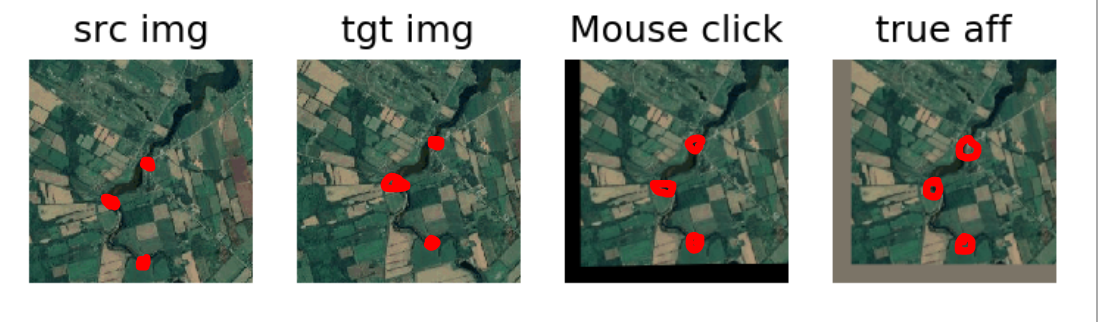
\includegraphics[width = 5.0in]{figs/click_20up_20right}
\caption{We pick 3 points from the source image(src) and 3 point from the target image(tgt) and generated the affine transformation from the points we picked(Mouse click) and compare it with  ground truth affine transformation(true aff).}
\end{figure}
  
 \begin{figure}
\centering
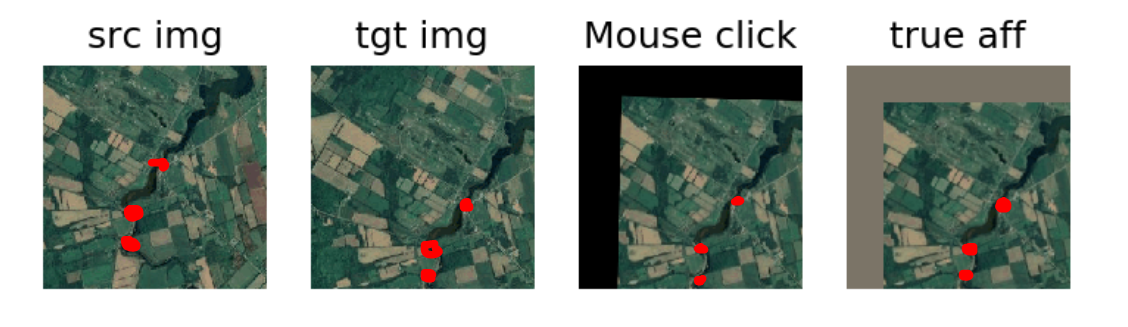
\includegraphics[width = 5.0in]{figs/click_40down_40right}
\caption{We pick 3 points from the source image(src) and 3 point from the target image(tgt) and generated the affine transformation from the points we picked(Mouse click) and compare it with  ground truth affine transformation(true aff).}
\end{figure}

\begin{figure}
\centering
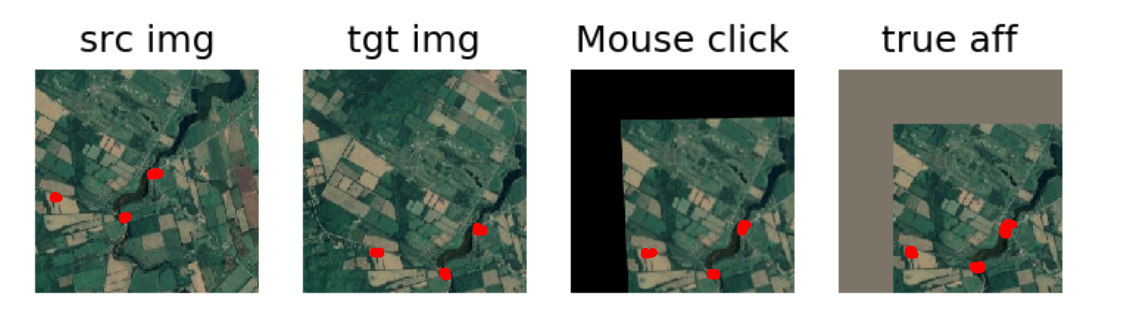
\includegraphics[width = 5.0in]{figs/click_60down_60right}
\caption{We pick 3 points from the source image(src) and 3 point from the target image(tgt) and generated the affine transformation from the points we picked(Mouse click) and compare it with  ground truth affine transformation(true aff).}
\end{figure}

\section{Result}
  We provided the many result examples in the previous section. Visually the model doesn't work well on large translations and the model fails when rotations are involved. In this section we numerically show the accuracy of the model in terms of MSE on our dataset of images. To emphasize the accuracy of the model we break our dataset down into the following subsets, which are chosen based on the degree of translation that they contain.
\begin{itemize}
\item data\_really\_small = A dataset that all the image pairs with translations of 60 or less and rotation.
\begin{itemize}
\item Total loss MSE (1320 images): 20.1473
\item Average loss per image: 0.0153.
\end{itemize}

\item  data\_small\_trans =A dataset that all the image pairs with rotation = 0 and translations of 80 or less.
\begin{itemize}
\item Total loss MSE (1760 images): 79.6672.
\item Average loss per image: 0.0453.
\end{itemize}

\item data\_no\_rot = A dataset that all the image pairs with rotation.
\begin{itemize}
\item Total loss MSE (2640 images):  286.9124.
\item Average loss per image:  0.1087.
\end{itemize}
\end{itemize}
  We can see compare the total loss MSE from these datasets, the data\_really\_small has the smallest error, when the translation is larger, the machine learning approach struggles to find the common features in the image pairsperiod. The model does not estimate large translations (those above 60 pixels) accuractely. In fact we can see in Figure 5.3 an example of this failing. The MSE for this individual example is 0.0735.
  % Experiment 2

\chapter{Observations and Conclusions}
This chapter will discuss the results of the model and the further study that could be done, also the impact of the training data and the limitation of the model.

 \section{Further research}
 This section we will discuss what could be done in the future so that the model will end up with better accuracy to estimate the affine transformation between the aerial images. We will address the research in terms of data and model.
\subsection{Data}
 We developed our own dataset for the purpose of training a machine learning model. However we only ended up using it to test a model that was trained with general images in the same manner as Rocco\cite{Rocco17}. We did try to train our model with this dataset however the model failed to converge. One thing we did not try was to train the model only on subsets of our dataset. Training it with the full set of data, including the rotations and large translations did not allow the model to become useful (the training error was too large). Only during testing and after visually inspecting some examples as we show in Chapter 5 did we develop some subsets of our dataset. It is possible the neural network would train using only our smaller datasets. We leave this for future work.\\
\begin{figure}
\centering
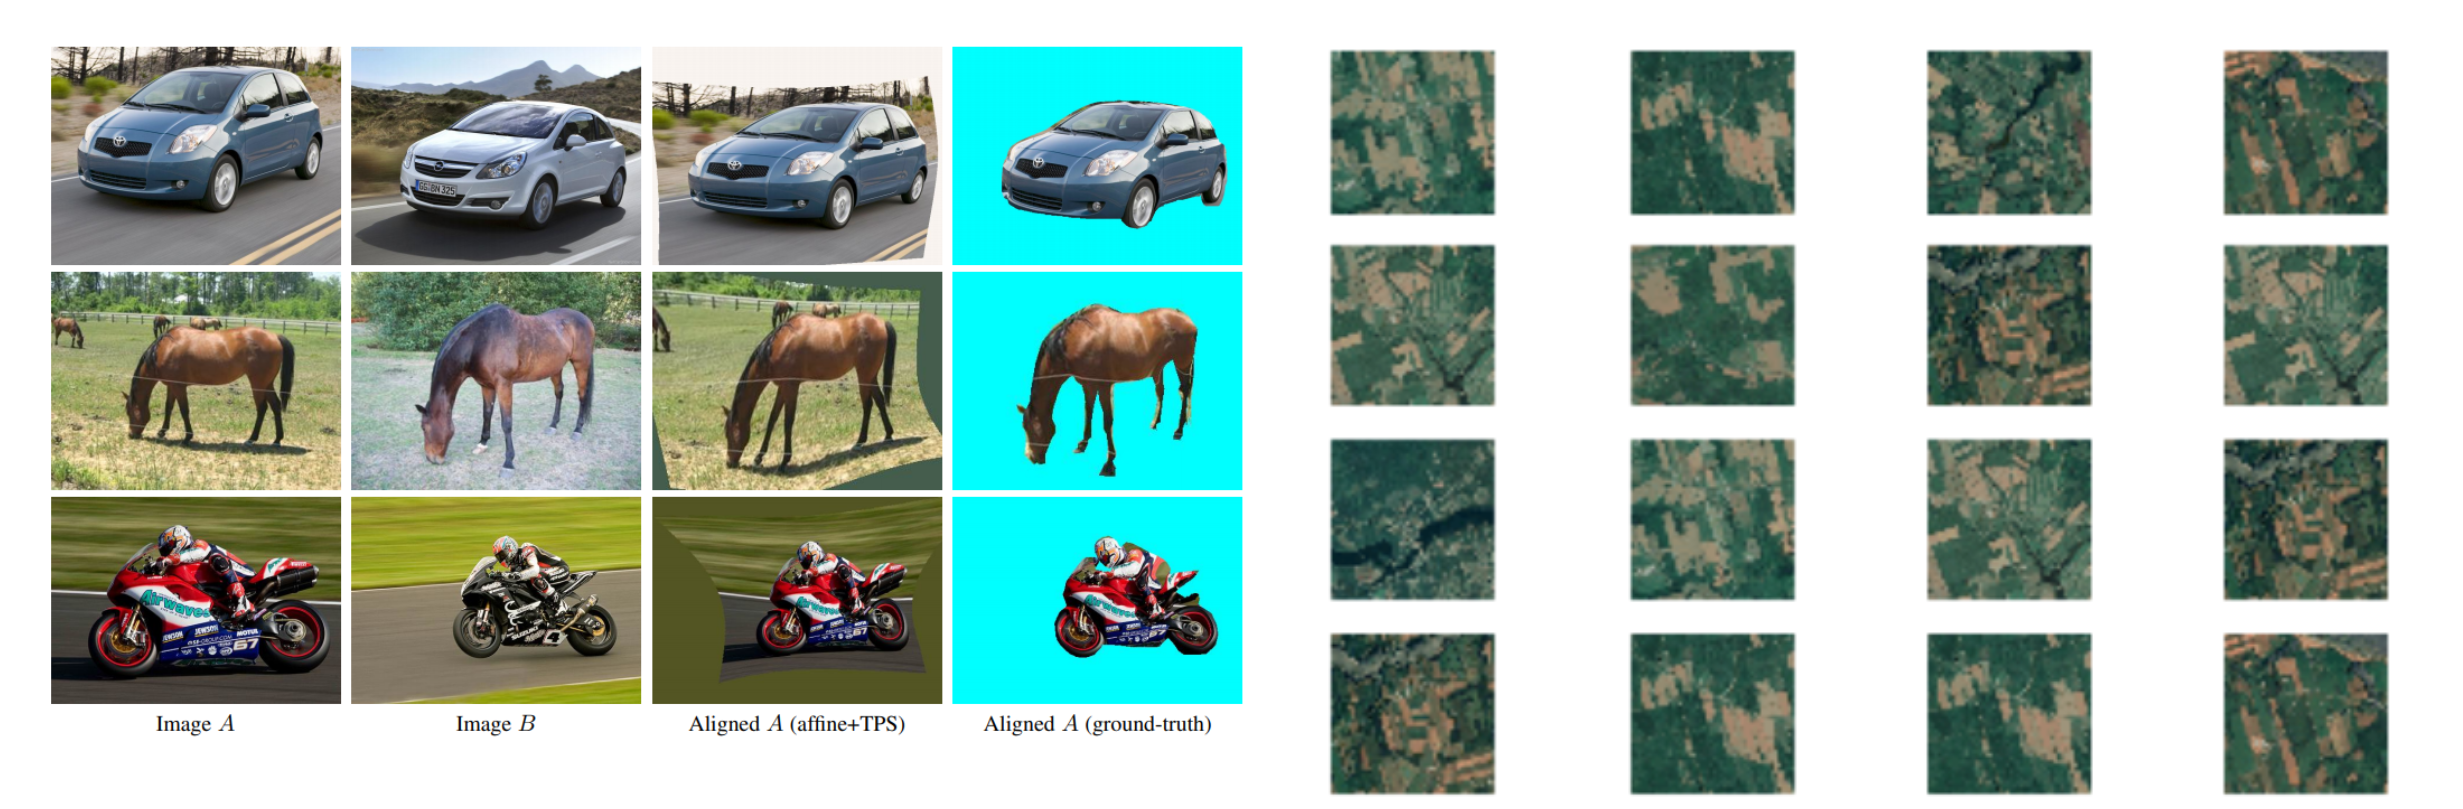
\includegraphics[width = 5.0in]{figs/data_compare}
\caption{The comparison of training data between Rooco,I\citep{Rocco17} and us. The training data from Rocco\citep{Rocco17}(left side) has some key features in the center of the images, but it is not too obvious what is the key features in our training images(right size).}
\end{figure}
 Other thing we could do when we develop the training dataset is try to keep the important feature in both source images and target image so that the model are not struggle finding the features in given image pairs. We developed over 10,000 image pairs to train the models, a datasets contains more than that is likely to help to train the model.
 Figure 6.2 shows one of our image pair that the target image are 60 pixels translate right and 60 pixels translate down.\\

\begin{figure}
\centering
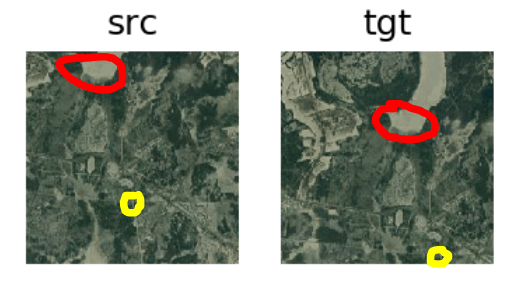
\includegraphics[width = 5.0in]{figs/train_src_tgr}
\caption{This shows a image pair, the target image are 60 pixels translate right and 60 pixels translate down. We circle out the common point in the images, we can see that it is very hard to find strong features between this image pairs even the translation is not too big.}
\end{figure}


\subsection{Model}
 We implement the model from Rocco.I\citep{Rocco17} to estimate only affine transform matrix, the model is working well to do the task, but it is possible to implement other machine learning models that may produce better results. We only implemented the one neural network, while a varied approach may have been beneficial.
\subsubsection{Loss function}
 We are using the MSE(Mean Square Error)\cite{mse} to calculate the error between the truth affine parameters $\theta_{af}$ and the predict affine parameters from the model $\theta_{pred}$.
  The advantage of the MSE is easy to implement and gives us the clear error for our affine transformation and $\theta_{af}$ and the predict affine parameters from the model $\theta_{pred}$. The MSE is a general loss function that works well and suitable for a lot of models for regression problems. \\
  The MSE is not specific for the model. In the model implement by Rocco,I\citep{Rocco17}, they develop the loss function by measuring loss on an imaginary grid of points which is being deformed by the transformation. The following section is form the paper "Convolutional neural network architecture for geometric matching" written by Ricco,I\citep{Rocco17} that gives a clear description of the loss function:
  \begin{quote}
  We construct a grid of points in image A, transform it using the ground truth and neural network estimated transformations $T_{\theta_{GT}}$ and $T_{\theta}$ with parameters $\theta_{GT}$ and $\theta$, respectively, and measure the discrepancy between the two transformed grids by summing the squared distances between the corresponding grid points:
  \begin{align*}
  L(\theta, \theta_{GT})= \frac{1}{N}\sum_{i=1}^{N}{d(T_{\theta}(g_i), T_{\theta_{GT}}(g_i) )}^2
  \end{align*}
  where $g = \{g_i\}=\{(x_i, y_i)\}$ is the uniform grid used, and N = |$g$|. We define the grid as having $x_i,y_i \in \{ s:\ s\ =\ -1\ +\ 0.1\ * n*n  \in \{0,1,2....,20 \} \}$, that is to say, each coordinate belongs to a partition of [-1,1] in equally spaced subintervals of steps 0.1. Note that we construct the coordinate system such that the center of the image is at (0,0) and that the width and height of the image are equal to 2,$i.e$. the bottom left and top right corners have coordinates (-1,-1) and (1,1), respectively.\\
   The gradient of the loss function with respect to the
transformation parameters, needed to perform backpropagation in order to learn network weights, can be computed easily if the location of the transformed grid points $T_{\theta}(g_i)$  is differentiable with respect to $\theta$. This is commonly the case, for example, when T is an affine transformation,
$T_{\theta}(g_i)$ is linear in parameters $\theta$ and therefore the loss can be differentiated in a straightforward manner.
\end{quote}   		
  We have tried to uses this loss function when we training the model with our own dataset, unfortunately just as with MSE, the model did not converge. Thus we were left with a model that did not perform the task. Given the ease of understanding with MSE we kept that cost function for our testing that we presented in Chapter 5

\section{Conclusion}
 We have described a network model that for estimate the affine transformation between the aerial images, the model work well when the source image and the target translation are within 40 pixels, when the image pairs translation go above 40 pixels or involve rotation, the machine learning are struggling produce accurate result.\\ 
   We see the opportunity to modify the training data to produce the better result or implement different model or loss function that the result could comes out more accurate.  % Results and Discussion

%\input{Chapters/Chapter7} % Conclusion

%% ----------------------------------------------------------------
% Now begin the Appendices, including them as separate files

\addtocontents{toc}{\vspace{2em}} % Add a gap in the Contents, for aesthetics

\appendix % Cue to tell LaTeX that the following 'chapters' are Appendices

%\chapter{An Appendix}

	% Appendix Title

%\input{Appendices/AppendixB} % Appendix Title

%\input{Appendices/AppendixC} % Appendix Title

\addtocontents{toc}{\vspace{2em}}  % Add a gap in the Contents, for aesthetics
\backmatter

%% ----------------------------------------------------------------
\label{Bibliography}
\lhead{\emph{Bibliography}}  % Change the left side page header to "Bibliography"
\bibliographystyle{unsrtnat}  % Use the "unsrtnat" BibTeX style for formatting the Bibliography
\bibliography{Bibliography}  % The references (bibliography) information are stored in the file named "Bibliography.bib"

\end{document}  % The End
%% ----------------------------------------------------------------